\documentclass{beamer}
\usepackage{csquotes}
\usepackage{tikz}
\usetikzlibrary{arrows,positioning,shapes.geometric, calc}
\usepackage{amsmath}
\usepackage{listings, xcolor}
\usepackage{lmodern}
\usepackage{adjustbox}
\usepackage{booktabs}
\usepackage{colortbl}
\usepackage{caption}
\usepackage{icomma}
\usepackage{bigstrut}
\usepackage{geometry}
\usepackage{subfigure}
\usepackage{algorithmic}


\DeclareMathOperator*{\argmin}{argmin}
\captionsetup[figure]{labelformat=empty}

\usetheme{metropolis}           % Use metropolis theme
\title{Neural Networks in Genetic Risk Prediction}
\date{\today}
\author{Robert M. Porsch}
\institute{Center for Genomic Science}
\begin{document}
\maketitle

\begin{frame}[t]{Introduction}
  Aim:
  \begin{itemize}
    \item Improve genetic risk prediction using Neural Networks
    \item Estimate non-linear effects
  \end{itemize}
  Models:
  \begin{itemize}
    \item Fully connected LD-layer with $L-1$ hidden layer
    \item Clumped connected LD-layer with $L-1$ hidden layers
    \item Convolutional NN with $L-1$ hidden layer
  \end{itemize}
\end{frame}

\section{Data preparation}

\begin{frame}[t]{Format of a bed file}
  Most commonly bed files are variant-major files
  \begin{itemize}
    \item Example: 00010000 are the genotypes of the SNP1 for 4 subjects
    \item Efficient if you want to single SNP associations
    \item Extremly inefficient if you want to do multiple regression
  \end{itemize}
  Solution:
  \begin{itemize}
    \item recode data from variant-major to sample-major
    \item Example: 00010000 would the the genotypes of 4 SNPs for 1 subjects
  \end{itemize}
  This allows efficient memory usage of stochastic gradient descent
\end{frame}

\begin{frame}[t]{Training, Development, Testing}
  \begin{columns}[t]
    \begin{column}{0.5\textwidth}
      Simulation Data 1:\\
      \begin{itemize}
        \item $\sim2,000$ samples
        \item 40 different simulated phenotypes
        \item based on 1000 Genome project
        \item $MAF\geq1\%$
      \end{itemize}
    \end{column}
    \begin{column}{0.5\textwidth}
     Simulation Data 2: 
     \begin{itemize}
       \item $\sim300,000$ samples
       \item 4 different simulated phenotypes
       \item based on UKB
        \item $MAF\geq1\%$
     \end{itemize}
    \end{column}
  \end{columns}
  Issues: sample size limitations for development/testing dataset \\
  I am currently only using the 1kG data.
\end{frame}

\section{Fully connected LD Layer}

\begin{frame}[t]{Architecture}
  \begin{columns}[t]
    \begin{column}{0.5\textwidth}
      Layer 1:
      \begin{algorithmic}
        \STATE initialize $Z$
        \FOR{v = LD-Blocks} 
        \STATE $z_v = W^{[1]}_vX_v$
        \STATE $a_v = g(z_v)$
        \STATE $APPEND(Z, z_v)$
        \ENDFOR
      \end{algorithmic}
      Layer $2$:\\
      \begin{itemize}
        \item fully connected layers to output
        \item $L_1$ regularization in $l=1,2$
        \item dropout with $p=0.8$
      \end{itemize}
    \end{column}
    \begin{column}{0.5\textwidth}
      Optimization:
      \begin{itemize}
        \item AdaGrad
        \item Mini-Batch gradient decent with $m=100$
        \item no early stopping ($epochs=100$)
        \item no hyper-parameter optimization (lambda, number of hidden layers)
      \end{itemize}
    \end{column}
  \end{columns}
\end{frame}

\begin{frame}[t]{Model Overview}
  \begin{figure}[htpb]
    \centering
    \includegraphics[width=0.8\linewidth]{./tensormodel.png}
  \end{figure}
\end{frame}

\begin{frame}[t]{Some results}
  \begin{figure}[htpb]
    \centering
    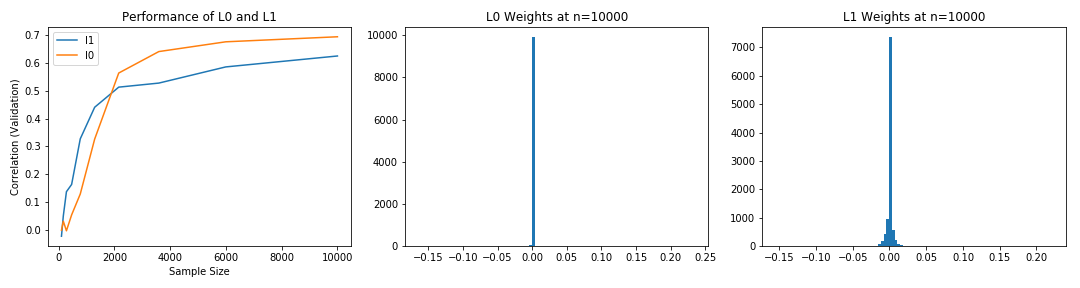
\includegraphics[width=0.8\linewidth]{performance.png}
    \caption{Example performance on phenotype 1}
  \end{figure}
  \begin{itemize}
    \item high variance problem
    \item disappointing performance in development set
    \item performance similar to LassoSum
  \end{itemize}
\end{frame}

\section{Clumped NN}

\begin{frame}[t]{Architecture}
  Similar architecture but with additional clumping step

  \begin{enumerate}[(i)]
    \item run GWAS on training set
    \item perform clumping ($r^2=0.5, p_1 = 0.01, p_2 = 0.1$) 
      \begin{itemize}
        \item Results in 72 SNPs
      \end{itemize}
    \item feed clumped genotype matrix into fully connected NN $L=3$
      \begin{itemize}
        \item $n^{[1]}_h=60, n^{[2]}_h=60, n^{[3]}_h=1$
        \item dropout layer after $l=1$ and $l=2$
      \end{itemize}
  \end{enumerate}
  No early stopping, ($epochs=100$), mini-batch with $m=100$
\end{frame}

\begin{frame}[t]{Results}
  \begin{figure}[htpb]
    \centering
    \includegraphics[width=0.8\linewidth]{./keras_model.png}
  \end{figure}
  \begin{itemize}
    \item Similar performance to the LD-connected NN
    \item high variance problem
  \end{itemize}
\end{frame}

\begin{frame}[t]{Conclusions}
  \begin{itemize}
    \item Stronger regularization is required
    \item Currently there is no hyper-parameter optimization
    \item Larger dataset should be used (requires some re-write of the data import)
    \item Current literature: More and more paper on penalized regression for genetic risk prediction (mostly Lasso)
  \end{itemize}
\end{frame}
\end{document}
